\documentclass[uplatex]{jsarticle}
\usepackage[utf8]{inputenc}

\usepackage{amsmath}
\usepackage[dvipdfmx]{graphicx}
\usepackage{resume}  % resume用スタイル
\usepackage{udline}  % 下線用
\usepackage{comment} % 複数行コメント
\pagestyle{plain}
 
\begin{document}
\twocolumn[
    \beginheader{令和5年度 コンピュータサイエンス学部 中間発表}{2023}{8}{9}{井上 研究室}
    \title{VR環境での落下感に姿勢が与える影響}
    \author{C0B20205 武田 夢音 (Yumene Takeda)}
    \endheader
]
\vspace{3mm}

%%ページ番号
\setcounter{page}{9}

\section{はじめに}

 
バーチャルリアリティ(VR)機器の高性能化・低廉化に伴い,一般消費者でもVR環境を用いて様々な体験をすることができるようになった.
VRは現実に近い体験をするために用いられることが多く,そのためには現実の再現によって起こる臨場感が必要である.しかし,一般的なVR機器は落下という感覚に対しての情報提示が視覚情報のみであり,一部のイベントでは風と人力での体位の変化を用いている場合があるが,落下感覚に影響を与える体位という要素を自動で変化させるデバイスの存在は耳にしない.

本研究では,伏臥位をとった体の角度を自動で変化させられるデバイスを開発し,落下時の体の角度および落下中の角度の変化が落下感覚に与える影響を明らかにすることを目的とする.

\begin{figure}[tb]
  % width や height で絶対的な大きさ指定をすることもできる
  \centering
  \fbox{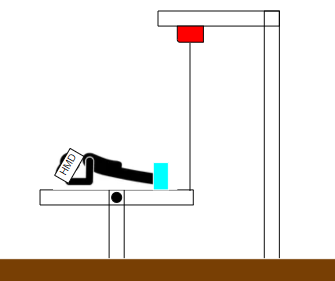
\includegraphics[width=1\linewidth]{fig/main_system.png}}
  \caption{システム概要図}
  \label{fig:about_system}

\end{figure}

\section{関連研究}
東山らの研究\cite{vection}はロールベクション(刺激によって反対方向に回転していると錯覚する効果)に姿勢が与える影響についての分析を行っており,被験者に5種類の体勢を取らせて視覚刺激を与えることで発生するベクションの強度や発生速度についての実験を行っている.結果から,ベクションの知覚が最も早くなるのはうつ伏せと仰向けであり,ベクションが筋肉系の活動状態(姿勢の制御)による影響を受けることが示された.

奥川らの研究\cite{spatial_stimulation_effect_falling}はVR空間における視覚刺激と体位によって発生する落下感覚の分析を行っており,落下時に見える風景の空間周波数と落下時の体位を数パターン用意し,それぞれの落下感覚を比較する実験を行った.結果から,空間周波数は高いほど落下感覚が高まり体位は伏臥位が最も落下感覚が高まるという結果が得られた.


 

\section{角度可変システム}
\subsection{システム概要}
システム概要の図を\figref{fig:about_system}に示す.プレイヤーは頭部にHMDを装着し,上から吊るされた台の上で伏臥位をとる.台の片側はウィンチにつながれており,VRシミュレーション中に体の角度を変えることができる.
仮想空間にはビルの上などの高い場所にいるシチュエーションを用意し,被験者に対して数百メートルの高さから落下する映像を提示できるようにする.
伏臥位になったプレイヤーはVR空間内で落下を体験し,落下に合わせて上下するウィンチによって体の角度が変化する.

\subsection{システム構成}
本研究で使用するウィンチはボタンによる操作を行うため,マイコンを用いてボタンを押すデバイスを作成し間接的に機械制御を行えるようにする.また,マイコンにはArudinoを用いる.

\section{評価方法}
本実験では落下感覚の比較のためマグニチュード法を用いる。

例えば基準となる状態での落下感覚を10として,比較を行いたい状態での落下感覚が半減したと感じたら5,倍程度になったと感じたら20と答えてもらう手法であり,数値にならない感覚の測定を行うのに適した手法である。

基準となる体位を水平な伏臥位として,そこから15度ずつ下に傾けた体位を比較対象として評価を行う。
また,実験中に角度を水平から傾けた際の落下感覚の変化も比較を行いたい。

\section{検討事項}
本研究の検討事項は3つある.

1つ目は落下時の風景である.落下時の風景は落下感覚に影響を与えることが明らかになっているため,本研究でも落下時に被験者に提示する風景は適したものにする必要がある.そこで,現状では先行研究で用いられていたビルからの落下もしくはランダムドットを用いて視覚刺激の空間周波数が高い風景にすることを検討している.

2つ目はシミュレーション中に体を傾ける場合,体を傾けるタイミングについてである.まだこのシミュレーション自体についての検討が足りていないため,体を傾けるタイミングやこのシミュレーション自体の必要性についても検討が必要である.

3つ目は安全性についてである.現在作成を考えているデバイスは体を固定する機構を想定しておらず,体を下に傾けすぎた場合にずり落ちてしまうことが容易に想像できる.また,角度の上下の際の安全性を考える必要もあるため,それらについて検討する必要がある.

\section{今後の展望}
まず目指すこととして,体を傾けることのできるデバイスが完成しておらず,実験に着手できないためその作成を第一の目標として作業を進める.

\section{まとめ}
本研究ではVR環境で落下する際の体位の角度の違いによって生じる落下感覚の差について比較と調査を行い,今後はデバイスの作成と実験を行う予定である.


 \bibliographystyle{junsrt}
\bibliography{ref.bib}   % 参考文献のデータベースファイルを指定する 
\end{document}
